\documentclass[tikz,border=0pt]{standalone}
\usepackage[american]{circuitikz}
\usetikzlibrary{arrows.meta,calc,positioning,decorations.pathmorphing,patterns}
\definecolor{zyloTeal}{HTML}{174A5B}
\definecolor{zyloTealTwo}{HTML}{246B7A}
\definecolor{zyloInk}{HTML}{1F2933}
\definecolor{zyloSoft}{HTML}{EAF4F4}
\definecolor{zyloPaper}{HTML}{F8FAFB}
\definecolor{zyloLine}{HTML}{44606B}
\definecolor{zyloOrange}{HTML}{D97706}
\begin{document}
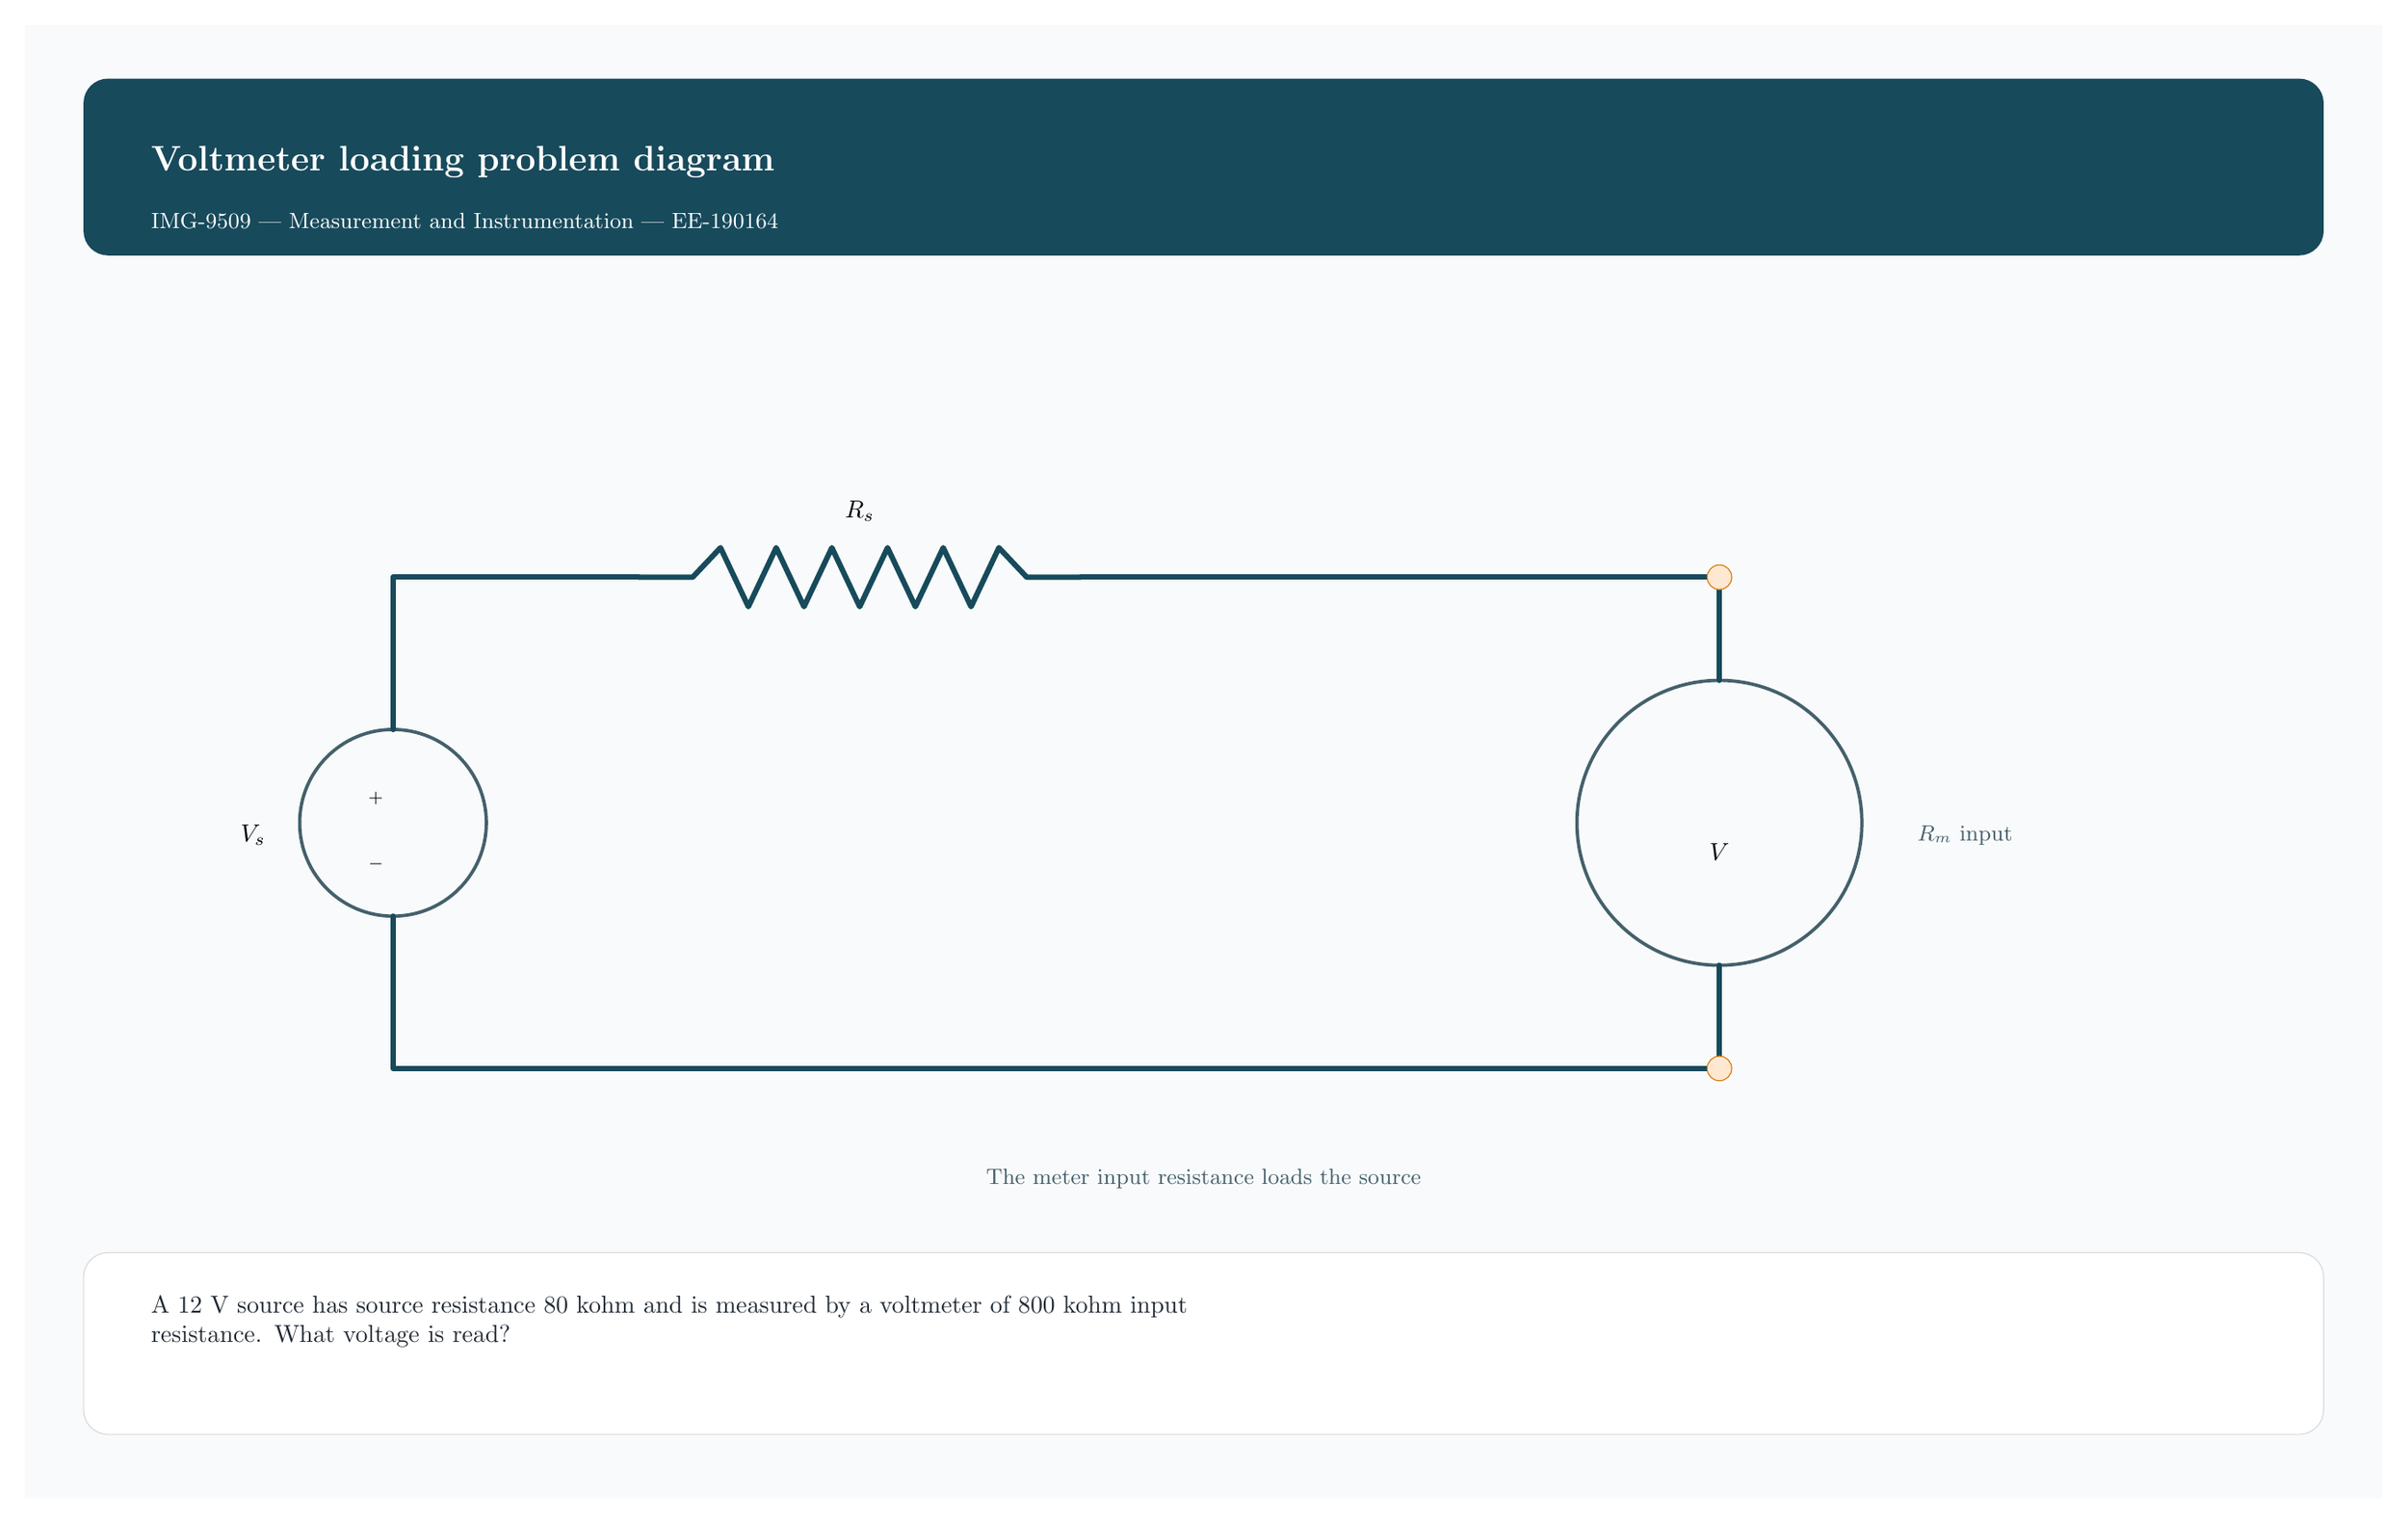
\begin{tikzpicture}[x=1pt,y=-1pt,>=Latex,line cap=round,line join=round]
\path[fill=zyloPaper] (0,0) rectangle (960,600);
\path[fill=zyloTeal,rounded corners=10pt] (24,22) rectangle (936,94);
\node[anchor=west,text=white,font=\bfseries\Large] at (48,56) {Voltmeter loading problem diagram};
\node[anchor=west,text=white!82,font=\small] at (48,80) {IMG-9509 | Measurement and Instrumentation | EE-190164};
\tikzset{wire/.style={draw=zyloTeal,line width=2.2pt},thinwire/.style={draw=zyloLine,line width=1.35pt},accent/.style={draw=zyloOrange,line width=2.2pt},box/.style={draw=zyloTealTwo,fill=zyloSoft,line width=1.5pt,rounded corners=8pt}}
\draw[thinwire] (150,325) circle (38); \node[font=\scriptsize] at (143,315) {$+$}; \node[font=\scriptsize] at (143,342) {$-$}; \node at (93,330) {$V_s$};
\draw[wire] (150,287) -- (150,225) -- (250,225);
\draw[wire] (250,225) -- (272,225) -- (272,225) -- (283.333,213) -- (294.667,237) -- (306,213) -- (317.333,237) -- (328.667,213) -- (340,237) -- (351.333,213) -- (362.667,237) -- (374,213) -- (385.333,237) -- (396.667,213) -- (408,225) -- (430,225);
\node at (340,198) {$R_s$}; \draw[wire] (430,225) -- (690,225);
\draw[thinwire] (690,325) circle (58); \node at (690,337) {$V$};
\draw[wire] (690,225) -- (690,267); \draw[wire] (690,383) -- (690,425) -- (150,425) -- (150,363);
\node[font=\small,text=zyloLine] at (790,330) {$R_m$ input};
\filldraw[draw=zyloOrange,fill=orange!18] (690,225) circle (5); \filldraw[draw=zyloOrange,fill=orange!18] (690,425) circle (5);
\node[font=\small,text=zyloLine] at (480,470) {The meter input resistance loads the source};
\path[draw=black!15,fill=white,rounded corners=10pt] (24,500) rectangle (936,574);
\node[anchor=west,text width=860pt,align=left,text=zyloInk,font=\normalsize] at (48,528) {A 12 V source has source resistance 80 kohm and is measured by a voltmeter of 800 kohm input\\resistance. What voltage is read?};
\end{tikzpicture}
\end{document}
